% New analysis update started from zero on 2026-08-20.
% Accepted P1--P3; scientific sources:
%   ../docs/progress.md
%   ../XGBoost/docs/knowledge/post_20260813_ml_delta_for_slides.md
%   ../Analysis_CODES/docs/slides_20260820_codes_delta.md
\documentclass[11pt,aspectratio=169]{beamer}

\usetheme{Madrid}
\usecolortheme{default}
\setbeamertemplate{navigation symbols}{}
\setbeamertemplate{footline}[frame number]

\usepackage{booktabs}
\usepackage{graphicx}
\usepackage{tikz}
\usetikzlibrary{arrows.meta,positioning}
\input{beamer_setup.tex}

% Optional fast single-frame build, e.g.:
%   bash fastcompile_frame.sh p2
\ifdefined\onlyframes
  \expandafter\includeonlyframes\expandafter{\onlyframes}
\fi

\definecolor{positive}{HTML}{0173B2}
\definecolor{negative}{HTML}{DE8F05}
\definecolor{emphasis}{HTML}{027A5A}
\definecolor{neutral}{HTML}{666666}
\setbeamercolor{structure}{fg=positive}
\setbeamercolor{block title}{fg=white,bg=positive}
\setbeamercolor{block body}{fg=black,bg=positive!8}
\setbeamercolor{block title alerted}{fg=white,bg=negative}
\setbeamercolor{block body alerted}{fg=black,bg=negative!10}
\setbeamercolor{block title example}{fg=white,bg=emphasis}
\setbeamercolor{block body example}{fg=black,bg=emphasis!8}
\newcommand{\pos}[1]{\textcolor{positive}{#1}}
\newcommand{\con}[1]{\textcolor{negative}{#1}}
\newcommand{\HL}[1]{\textcolor{emphasis}{#1}}
\newcommand{\muted}[1]{\textcolor{neutral}{#1}}

\title[X(3872) Analysis Update]{X(3872) Analysis Update}
\subtitle{PbPb $\psi(2S)$ validation and the PbPb23 X extension}
\author{%
  Henrique Legoinha, \underline{Lekai Yao}, Nuno Leonardo, Zhen Hu\\[0.45em]
  2026.8.20%
}
\institute{}
\date{%
  \includegraphics[height=1.653cm]{figures/symbols/CERN.png}\hspace{0.30cm}%
  \includegraphics[height=1.653cm]{figures/symbols/CMS.png}\hspace{0.30cm}%
  \includegraphics[height=1.653cm]{figures/symbols/LIP.png}\hspace{0.30cm}%
  \includegraphics[height=1.653cm]{figures/symbols/LU.png}\hspace{0.30cm}%
  \includegraphics[height=1.653cm]{figures/symbols/THU.png}%
}

\begin{document}

\begin{frame}[plain,label=p1]
  \titlepage
\end{frame}

\begin{frame}[label=p2]{Recap: where the previous update stopped}
  \small
  \centering
  \vspace{0.25em}
  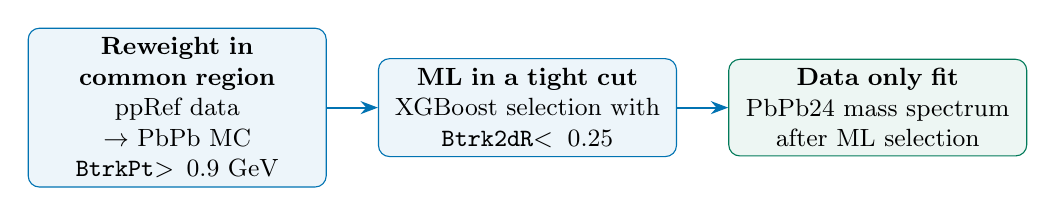
\begin{tikzpicture}[
    node distance=0.65cm,
    flowbox/.style={draw=positive,rounded corners,fill=positive!7,
      text width=3.55cm,minimum height=1.05cm,align=center,font=\small},
    last/.style={draw=emphasis,rounded corners,fill=emphasis!7,
      text width=3.55cm,minimum height=1.05cm,align=center,font=\small},
    arr/.style={-{Stealth[length=2.2mm]},thick,positive}
  ]
    \node[flowbox] (a) {\textbf{Reweight in common region}\\ppRef data $\rightarrow$ PbPb MC\\\texttt{BtrkPt}$>0.9$ GeV};
    \node[flowbox,right=of a] (b) {\textbf{ML in a tight cut}\\XGBoost selection with\\\texttt{Btrk2dR}$<0.25$};
    \node[last,right=of b] (c) {\textbf{Data only fit}\\PbPb24 mass spectrum\\after ML selection};
    \draw[arr] (a)--(b);
    \draw[arr] (b)--(c);
  \end{tikzpicture}

  \vspace{0.65em}
  \begin{columns}[T,onlytextwidth]
    \begin{column}{0.48\textwidth}
      \begin{exampleblock}{Established}
        \begin{itemize}
          \item ppRef and PbPb X MC are close in the same fiducial region.
          \item A X(3872) peak appears in PbPb after ML.
        \end{itemize}
      \end{exampleblock}
    \end{column}
    \begin{column}{0.48\textwidth}
      \begin{alertblock}{Still open}
        \begin{itemize}
          \item Better reweighting \& selection need more study.
          \item 2023 PbPb data could be added.
        \end{itemize}
      \end{alertblock}
    \end{column}
  \end{columns}
\end{frame}

\begin{frame}[label=p3]{Updates from last week}
  \small
  \centering
  \vspace{0.20em}
  \begin{columns}[T,onlytextwidth]
    \begin{column}{0.48\textwidth}
      \centering
      {\large\bfseries $\psi(2S)$ ppRef weight $\rightarrow$ PbPb}\par
      \vspace{0.35em}
      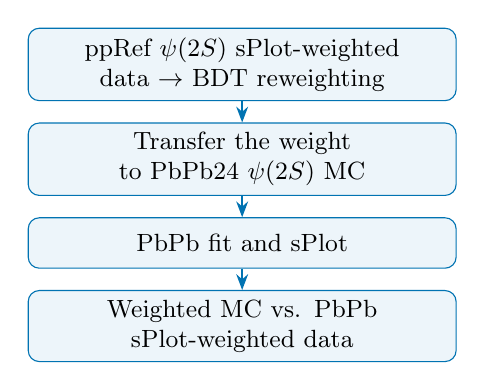
\begin{tikzpicture}[
        node distance=0.27cm,
        route/.style={draw=positive,rounded corners,fill=positive!7,
          text width=5.20cm,minimum height=0.64cm,align=center,font=\small},
        arr/.style={-{Stealth[length=2mm]},thick,positive}
      ]
        \node[route] (a) {ppRef $\psi(2S)$ sPlot-weighted data $\rightarrow$ BDT reweighting};
        \node[route,below=of a] (b) {Transfer the weight to PbPb24 $\psi(2S)$ MC};
        \node[route,below=of b] (c) {PbPb fit and sPlot};
        \node[route,below=of c] (d) {Weighted MC vs. PbPb sPlot-weighted data};
        \draw[arr] (a)--(b); \draw[arr] (b)--(c); \draw[arr] (c)--(d);
      \end{tikzpicture}
      \vspace{0.35em}
      \begin{beamercolorbox}[wd=0.95\linewidth,sep=0.35em,center,rounded=true]{block body}
        \textbf{Question:} can PbPb data validate the transferred weight?
      \end{beamercolorbox}
    \end{column}

    \begin{column}{0.48\textwidth}
      \centering
      {\large\bfseries Add PbPb23 to the X fit}\par
      \vspace{0.35em}
      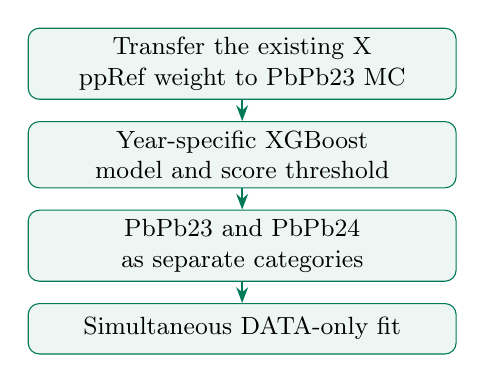
\begin{tikzpicture}[
        node distance=0.27cm,
        route/.style={draw=emphasis,rounded corners,fill=emphasis!7,
          text width=5.20cm,minimum height=0.64cm,align=center,font=\small},
        arr/.style={-{Stealth[length=2mm]},thick,emphasis}
      ]
        \node[route] (a) {Transfer the existing X ppRef weight to PbPb23 MC};
        \node[route,below=of a] (b) {Year-specific XGBoost model and score threshold};
        \node[route,below=of b] (c) {PbPb23 and PbPb24 as separate categories};
        \node[route,below=of c] (d) {Simultaneous DATA-only fit};
        \draw[arr] (a)--(b); \draw[arr] (b)--(c); \draw[arr] (c)--(d);
      \end{tikzpicture}
      \vspace{0.35em}
      \begin{beamercolorbox}[wd=0.95\linewidth,sep=0.35em,center,rounded=true]{block body example}
        \textbf{Question:} does the added year materially strengthen the result?
      \end{beamercolorbox}
    \end{column}
  \end{columns}
\end{frame}

\begin{frame}[label=p4]{$\psi(2S)$ reweighting, ML and fit configuration}
  \footnotesize
  \begin{columns}[T,onlytextwidth]
    \begin{column}{0.33\textwidth}
      \textbf{Common region}
      \begin{itemize}
        \setlength{\itemsep}{0.08em}
        \item $10<\texttt{Bpt}<50$ GeV
        \item $|\texttt{By}|<1.6$, $\texttt{BQvalue}<0.15$
        \item $0.9<\texttt{Btrk1Pt},\texttt{Btrk2Pt}\leq4.5$ GeV
        \item $2<\texttt{Btktkpt}\leq8$ GeV
        \item $\texttt{Btrk1dR}\leq0.45$
        \item $\texttt{Btrk2dR}\leq0.25$
      \end{itemize}
    \end{column}
    \begin{column}{0.30\textwidth}
      \textbf{Reweighting variables}
      \begin{itemize}
        \setlength{\itemsep}{0.08em}
        \item \texttt{Bcos\_dtheta}
        \item \texttt{Btktkpt}
        \item \texttt{Bchi2Prob}
        \item \texttt{Btrk2Pt}
        \item \texttt{Btrk1Pt}
        \item \texttt{Btrk1dR}
      \end{itemize}
    \end{column}
    \begin{column}{0.33\textwidth}
      \textbf{ML training samples}
      \begin{itemize}
        \setlength{\itemsep}{0.08em}
        \item Signal: reweighted PbPb24 $\psi(2S)$ MC
        \item Background: PbPb24 DATA sidebands
        \item $3.60<m<3.65$ or $3.75<m<3.80$ GeV
        \item Same common region
      \end{itemize}
      \textbf{ML variables}\\[0.10em]
      \texttt{Btrk1dR}, \texttt{Btktkpt}, \texttt{Btrk1Pt},\\
      \texttt{Bchi2Prob}, \texttt{Bcos\_dtheta}, \texttt{Btrk2Pt}
    \end{column}
  \end{columns}

  \vspace{0.35em}
  \begin{block}{DATA-only fit model}
    \centering
    Extended unbinned fit in $3.60<m<3.80$ GeV: single Gaussian signal + second-order Chebyshev background.\\[0.20em]
    $\mu$ starts at $3.686097$ GeV and floats within $\pm5$ MeV;
    $1\leq\sigma\leq8$ MeV.
  \end{block}
\end{frame}

\begin{frame}[label=p5]{PbPb $\psi(2S)$ DATA-only fits}
  \small
  \begin{columns}[T,onlytextwidth]
    \begin{column}{0.49\textwidth}
      \centering
      \includegraphics[width=0.87\linewidth]{../Analysis_CODES/fitER/results/manifest_driven_psi2s_data_gaussian/Psi2S_pb24_v1_fid1_6v1_rwr6range4v1_xgb_v1/data_gaussian_pdgfloat_v1/psi2seff30/data_fit.pdf}
      \vspace{-0.55em}
      \begin{tabular}{lr}
        signal efficiency & 30\% \\
        fitted yield & $86.10\pm20.78$ \\
        mean / $\sigma$ & $3.68597$ GeV / $2.97$ MeV \\
        status / covQual & $0/3$ \\
      \end{tabular}
    \end{column}
    \begin{column}{0.49\textwidth}
      \centering
      \includegraphics[width=0.87\linewidth]{../Analysis_CODES/fitER/results/psi2s_high_efficiency_exploratory/Psi2S_pb24_v1_fid1_6v1_rwr6range4v1_xgb_v1/xeff45_70_data_gaussian_v1/psi2seff45/data_fit.pdf}
      \vspace{-0.55em}
      \begin{tabular}{lr}
        signal efficiency & 45\% \\
        fitted yield & $150.90\pm36.59$ \\
        mean / $\sigma$ & $3.68600$ GeV / $3.71$ MeV \\
        status / covQual & $0/3$ \\
      \end{tabular}
    \end{column}
  \end{columns}
\end{frame}

\begin{frame}[label=p6]{sPlot-weighted PbPb DATA vs reweighted MC}
  \small
  \begin{columns}[T,onlytextwidth]
    \begin{column}{0.49\textwidth}
      \centering
      \textbf{In-model example: \texttt{Bcos\_dtheta}}\\[-0.25em]
      \includegraphics[width=0.84\linewidth]{../Analysis_CODES/plotER/Validation/results/pbpb24_psi2s_splot_validation/Psi2S_pb24_v1_fid1_6v1_rwr6range4v1_xgb_v1/xeff30_nominal_v2_lowneff_results_v2/variables/Bcos_dtheta/comparison.pdf}
      \vspace{-0.45em}
      weighted CDF distance $=0.190$\\
      used in the reweighting model
    \end{column}
    \begin{column}{0.49\textwidth}
      \centering
      \textbf{Held-out example: \texttt{Btrk2dR}}\\[-0.25em]
      \includegraphics[width=0.84\linewidth]{../Analysis_CODES/plotER/Validation/results/pbpb24_psi2s_splot_validation/Psi2S_pb24_v1_fid1_6v1_rwr6range4v1_xgb_v1/xeff30_nominal_v2_lowneff_results_v2/variables/Btrk2dR/comparison.pdf}
      \vspace{-0.45em}
      weighted CDF distance $=0.254$\\
      not used for reweighting; tests reliability on other variables
    \end{column}
  \end{columns}
\end{frame}

\begin{frame}[label=p7]{All 12 comparisons at xeff30}
  \footnotesize
  \vspace{0.15em}
  \begin{columns}[T,onlytextwidth]
    \begin{column}{0.49\textwidth}
      \centering
      \textbf{In-model reweighting variables}\\[0.15em]
      \renewcommand{\arraystretch}{1.15}
      \begin{tabular}{lrr}
        \toprule
        variable & before RW & after RW \\
        \midrule
        \texttt{Bcos\_dtheta} & 0.349 & 0.190 \\
        \texttt{Btktkpt}      & 0.232 & 0.212 \\
        \texttt{Bchi2Prob}     & 0.129 & 0.175 \\
        \texttt{Btrk2Pt}       & 0.066 & 0.056 \\
        \texttt{Btrk1Pt}       & 0.139 & 0.128 \\
        \texttt{Btrk1dR}       & 0.048 & 0.032 \\
        \bottomrule
      \end{tabular}
    \end{column}
    \begin{column}{0.49\textwidth}
      \centering
      \textbf{Held-out transfer variables}\\[0.15em]
      \renewcommand{\arraystretch}{1.15}
      \begin{tabular}{lrr}
        \toprule
        variable & before RW & after RW \\
        \midrule
        \texttt{Btrk2dR}   & 0.252 & 0.254 \\
        \texttt{BtrkPtimb}  & 0.144 & 0.147 \\
        \texttt{BtktkvProb} & 0.159 & 0.130 \\
        \texttt{Bpt}        & 0.134 & 0.128 \\
        $|\texttt{By}|$     & 0.104 & 0.114 \\
        \texttt{BQvalue}    & 0.204 & 0.211 \\
        \bottomrule
      \end{tabular}
    \end{column}
  \end{columns}

  \vfill
  \centering
  \begin{beamercolorbox}[wd=0.94\textwidth,sep=0.38em,center,rounded=true]{block body alerted}
    $N_{\rm eff}=(\sum w)^2/\sum w^2$ measures the statistical power left after signed-weight
    cancellation. Here $N_{\rm eff}=26.7$ is small, so the sPlot-weighted DATA shapes are not yet
    reliable enough to validate the transfer.
  \end{beamercolorbox}
\end{frame}

\begin{frame}[label=p8]{Why the $\psi(2S)$ validation stopped}
  \footnotesize
  \centering
  \renewcommand{\arraystretch}{1.15}
  \begin{tabular}{lrr}
    \toprule
    quantity & xeff30 & xeff45 one-off \\
    \midrule
    score cut & 0.898424 & 0.794011 \\
    selected DATA entries & 3197 & 9434 \\
    DATA-only fitted yield & $86.10\pm20.78$ & $150.90\pm36.59$ \\
    signed sPlot sum & 86.013 & 150.996 \\
    $\sum w^2$ & 277.149 & 870.049 \\
    signed $N_{\rm eff}=(\sum w)^2/\sum w^2$ & \textbf{26.694} & \textbf{26.205} \\
    negative-weight fraction & 89.115\% & 88.616\% \\
    variable-comparison execution & 12/12, low-$N_{\rm eff}$ override & 0/12, gate stop \\
    \bottomrule
  \end{tabular}

  \vspace{0.30em}
  \begin{columns}[T,onlytextwidth]
    \begin{column}{0.48\textwidth}
      \begin{exampleblock}{Established}
        RW, migration, ML, fit and sPlot interfaces are operational.
      \end{exampleblock}
    \end{column}
    \begin{column}{0.48\textwidth}
      \begin{alertblock}{Current limitation}
        Loosening to xeff45 increases candidates and yield, but does not improve signed $N_{\rm eff}$.
      \end{alertblock}
    \end{column}
  \end{columns}

  \vfill
  \centering\bfseries
  Physics validation remains statistics-limited and inconclusive.
\end{frame}

\begin{frame}[label=p9]{Adding PbPb23: reweighting, ML and fit configuration}
  \scriptsize
  \begin{columns}[T,onlytextwidth]
    \begin{column}{0.32\textwidth}
      \textbf{ppRef-derived reweighting}
      \begin{itemize}
        \setlength{\itemsep}{0.08em}
        \item Original: ppRef X MC
        \item Target: ppRef X sPlot-weighted DATA
        \item Same weight applied separately to PbPb23 and PbPb24 X MC
      \end{itemize}
      \textbf{Variables}\\[-0.10em]
      \texttt{Bcos\_dtheta}, \texttt{Btktkpt},\\
      \texttt{Bchi2Prob}, \texttt{Btrk2Pt},\\
      \texttt{Btrk1Pt}, \texttt{Btrk1dR}

      \vspace{0.20em}
      \textbf{RW region}\\[-0.10em]
      $10<\texttt{Bpt}<50$ GeV, $|\texttt{By}|<1.6$,\\
      $\texttt{BQvalue}<0.15$, $\texttt{BtrkPt}>0.9$ GeV,\\
      $2\leq\texttt{Btktkpt}\leq8$ GeV,\\
      $\texttt{Btrk1dR}\leq0.45$, $\texttt{Btrk2dR}\leq0.40$
    \end{column}

    \begin{column}{0.33\textwidth}
      \textbf{Year-specific ML training}
      \begin{itemize}
        \setlength{\itemsep}{0.08em}
        \item Signal: reweighted X MC of the same year
        \item Background: DATA in $[3.82,3.85]\cup[3.89,3.92]$ GeV
        \item Separate PbPb23 and PbPb24 classifiers
        \item test AUC: $0.89756/0.89587$
      \end{itemize}
      \textbf{Variables}\\[-0.10em]
      \texttt{Btrk1dR}, \texttt{Btktkpt}, \texttt{Btrk1Pt},\\
      \texttt{Bchi2Prob}, \texttt{Bcos\_dtheta}, \texttt{Btrk2Pt}

      \vspace{0.20em}
      \textbf{ML and fit region}\\[-0.10em]
      Same as above, but $\texttt{Btrk2dR}<0.25$.\\
      Year-specific score thresholds at common weighted X efficiency.
    \end{column}

    \begin{column}{0.31\textwidth}
      \textbf{Simultaneous DATA-only fit}
      \begin{itemize}
        \setlength{\itemsep}{0.08em}
        \item PbPb23 and PbPb24 are separate categories
        \item Extended unbinned fit in $3.80<m<3.94$ GeV
        \item Single Gaussian signal
        \item Shared mean: $3.86<\mu<3.88$ GeV
        \item Independent widths: $2\leq\sigma\leq8$ MeV
        \item Independent yields and Chebyshev-2 backgrounds
      \end{itemize}

      \vspace{0.20em}
      \begin{beamercolorbox}[wd=\linewidth,sep=0.40em,center,rounded=true]{block body example}
        Same RW--ML--fit chain for both years; only the year category and trained classifier differ.
      \end{beamercolorbox}
    \end{column}
  \end{columns}
\end{frame}

\begin{frame}[label=p10]{PbPb23 and PbPb24 simultaneous fits at xeff25}
  \small
  \begin{columns}[T,onlytextwidth]
    \begin{column}{0.49\textwidth}
      \centering
      \includegraphics[height=0.55\textheight]{../Analysis_CODES/fitER/results/pbpb_x_simultaneous_year_fit/X_pb23_v3_fid3_6v5_rwr6range5v1_xgb_v1/phase1_sqrtq0_v1/xeff25/pb23_fit.pdf}

      \vspace{0.15em}
      \begin{tabular}{lr}
        selected candidates & 972 \\
        score threshold & 0.952613 \\
        fitted yield & $29.03\pm19.29$ \\
        Gaussian width & $8.000$ MeV [upper bound] \\
      \end{tabular}
    \end{column}
    \begin{column}{0.49\textwidth}
      \centering
      \includegraphics[height=0.55\textheight]{../Analysis_CODES/fitER/results/pbpb_x_simultaneous_year_fit/X_pb23_v3_fid3_6v5_rwr6range5v1_xgb_v1/phase1_sqrtq0_v1/xeff25/pb24_fit.pdf}

      \vspace{0.15em}
      \begin{tabular}{lr}
        selected candidates & 870 \\
        score threshold & 0.953525 \\
        fitted yield & $58.67\pm18.68$ \\
        Gaussian width & $8.000$ MeV [upper bound] \\
      \end{tabular}
    \end{column}
  \end{columns}

  \vfill
  \centering
  Shared fitted mean: $3.87133$ GeV; fit status / covQual: $0/3$.
\end{frame}

\begin{frame}[label=p11]{X fit scan after adding PbPb23}
  \scriptsize
  \centering
  \includegraphics[width=0.72\textwidth,trim=0 0 0 15,clip]{../Analysis_CODES/fitER/results/pbpb_x_simultaneous_year_fit/X_pb23_v3_fid3_6v5_rwr6range5v1_xgb_v1/phase1_sqrtq0_v1/fit_scan_summary.pdf}

  \vspace{-0.30em}
  \renewcommand{\arraystretch}{1.00}
  \begin{tabular}{lccccccc}
    \toprule
    target weighted X efficiency & 10\% & 15\% & 20\% & 25\% & 30\% & 35\% & 40\% \\
    \midrule
    significance & 3.303 & 2.764 & 3.396 & 3.578 & 2.331 & 0.891 & 2.143 \\
    \bottomrule
  \end{tabular}

  \vspace{0.12em}
  \begin{columns}[T,onlytextwidth]
    \begin{column}{0.48\textwidth}
      \begin{beamercolorbox}[wd=\linewidth,sep=0.32em,rounded=true]{block body example}
        \textbf{Matched xeff25 comparison}\quad
        PbPb24-only: $3.247$; two-year joint: $3.578$; change: $+0.33$.
      \end{beamercolorbox}
    \end{column}
    \begin{column}{0.48\textwidth}
      \begin{beamercolorbox}[wd=\linewidth,sep=0.32em,rounded=true]{block body alerted}
        \textbf{Interpretation}\quad The change is modest. Uncalibrated local likelihood proxy;
        both widths hit the upper bound.
      \end{beamercolorbox}
    \end{column}
  \end{columns}
\end{frame}

\begin{frame}[label=p12]{Summary and Outlook}
  \small
  \begin{block}{Summary}
    \begin{itemize}
      \setlength{\itemsep}{0.35em}
      \item The $\psi(2S)$ workflow is working.
      \item The available $\psi(2S)$ statistics limit the validation of the reweighted MC variables.
      \item PbPb23 data have been added to the X ppRef$\rightarrow$PbPb analysis, with preliminary fit results.
      \item The PbPb23 data provide only a small increase in significance.
    \end{itemize}
  \end{block}

  \vspace{0.35em}
  \begin{exampleblock}{Outlook}
    \begin{itemize}
      \setlength{\itemsep}{0.30em}
      \item Better reweighting and selection need more study.
      \item A physics-approved configuration is needed before a calibrated significance study.
    \end{itemize}
  \end{exampleblock}
\end{frame}

\begin{frame}[plain,label=p13]{\strut}
  \centering
  \vfill
  \makebox[\textwidth][c]{%
    \begin{beamercolorbox}[wd=0.68\textwidth,sep=1.2em,center,rounded=true,shadow=true]{block body}
      {\LARGE\bfseries Thanks for listening!}\par
      \vspace{1.0em}
      {\large Reporter: Lekai Yao}\par
      \vspace{0.45em}
      {\large 2026.8.20}
    \end{beamercolorbox}%
  }
  \vfill
\end{frame}

\end{document}
